\begin{titlepage}
%	\includepdf[pages=-]{front_cover.pdf}

% The easiest way to cope with RuG font requirements is just use your favorite text editor (word, libre) and export that to PDF. Remember to set your page to B5! There's a .doc file attached.
	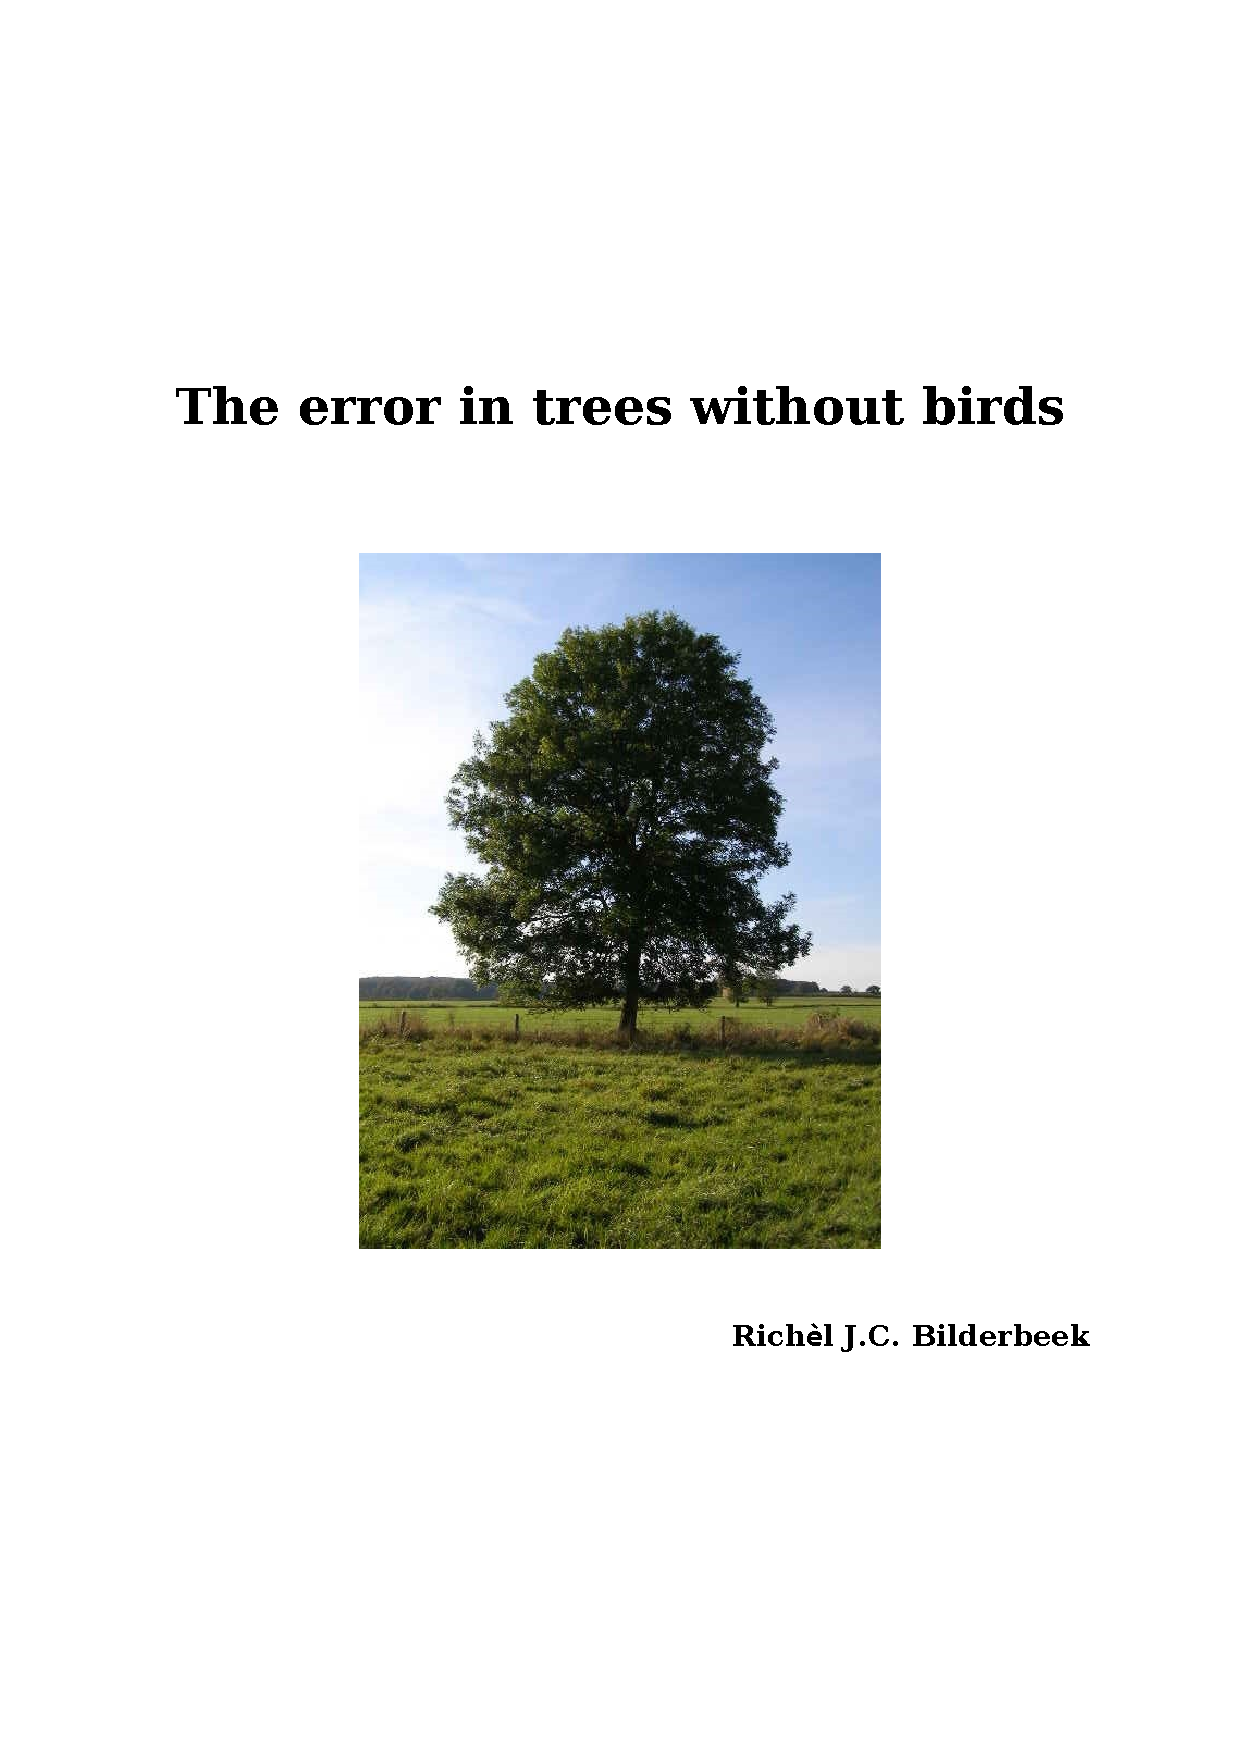
\includepdf[pages=-]{title/firstpage.pdf}
	
	
	%%%%%%%%%%%%%%%%%%%%%%%%%%%%% Book information page %%%%%%%%%%%%%%%%%%%%%%%%%%%%%%%%%%%%%
	
	\newpage \thispagestyle{empty}
	\vspace*{3.9cm}%{4.7cm} was 5.7, save 2 for FSC logo
	
	
	\begin{figure}[!h]
		
\includegraphics[width=\textwidth]{images/frontmatter/zernike.pdf}
	\end{figure}
	
	\vfill
	\begin{figure}[!h]
		
\includegraphics[width=\textwidth]{images/frontmatter/all-logos.pdf}
	\end{figure}
	\noindent
	{\small 
		Zernike Institute PhD thesis series 2016-12 \\
		ISSN:   1570-1530\\
		ISBN:	978-90-367-8806-9 \\
		ISBN:   978-90-367-8805-2 (electronic version) \\
		\\
		The work described in this thesis was performed in the research group Single Molecule Biophysics of the Zernike Institute for Advanced Materials at the University of Groningen, the Netherlands. \\
		\\
		Cover design: Rich\`el J.C. Bilderbeek\\
		Cover image: Super-resolution image reconstruction o \textit{E. coli} cells. Membrane marker (red) is LacY-eYFP and blue is UmuC-mKate2.
		\\
			%	An electronic version of this dissertation is available at: \\
	%	\url{http://MYTHESIS.COM}
		Printed by: GVO drukkers \& vormgevers B.V. \\
		} 	
	
	
	\clearpage
	
	
\includepdf[pages=-]{title/titlepage.pdf}
	
\end{titlepage}
